\section{Goal Design}
As mentioned in the beginning of this report, the major influencer for the goal design is the battery consumption. We presented our findings on how much battery each goal component uses in the chapter Tests and in this chapter draw conclusions for the actual goal design.

The power consumption of each component is quite significant. Together, the laser  and sensor consume $28.5mA$ while the esp32 consumes $80mA$ during computation intensive tasks and $20mA$ in idle. Letting the lasers run all the time is thus similar to letting the esp32 run on idle all time. Doing the former makes little sense though and booting up the esp32 more than needed is also a waste of power. So a well defined balance is needed and optimally, one which adapts to the usage pattern of the foosball table.  Thus, our goal is to make the goal smart and the esp32 has a hold function for its pins that enables us to do excatly that. The function \textit{esp\_err\_trtc\_gpio\_hold\_en(gpio\_num\_tgpio\_num)} holds the current on a specific port even when the esp32 goes into deepsleep\cite{GPIORTCG11esp32letPinsOn:online}.

This allows us to control a transistor even when the esp32 is in deepsleep. The laser and sensor are still directly powered from the battery, but the esp32 has full control over it. \Cref{fig:smartGoalDesign} shows this new setup.

\begin{figure}[h!]
    \centering
    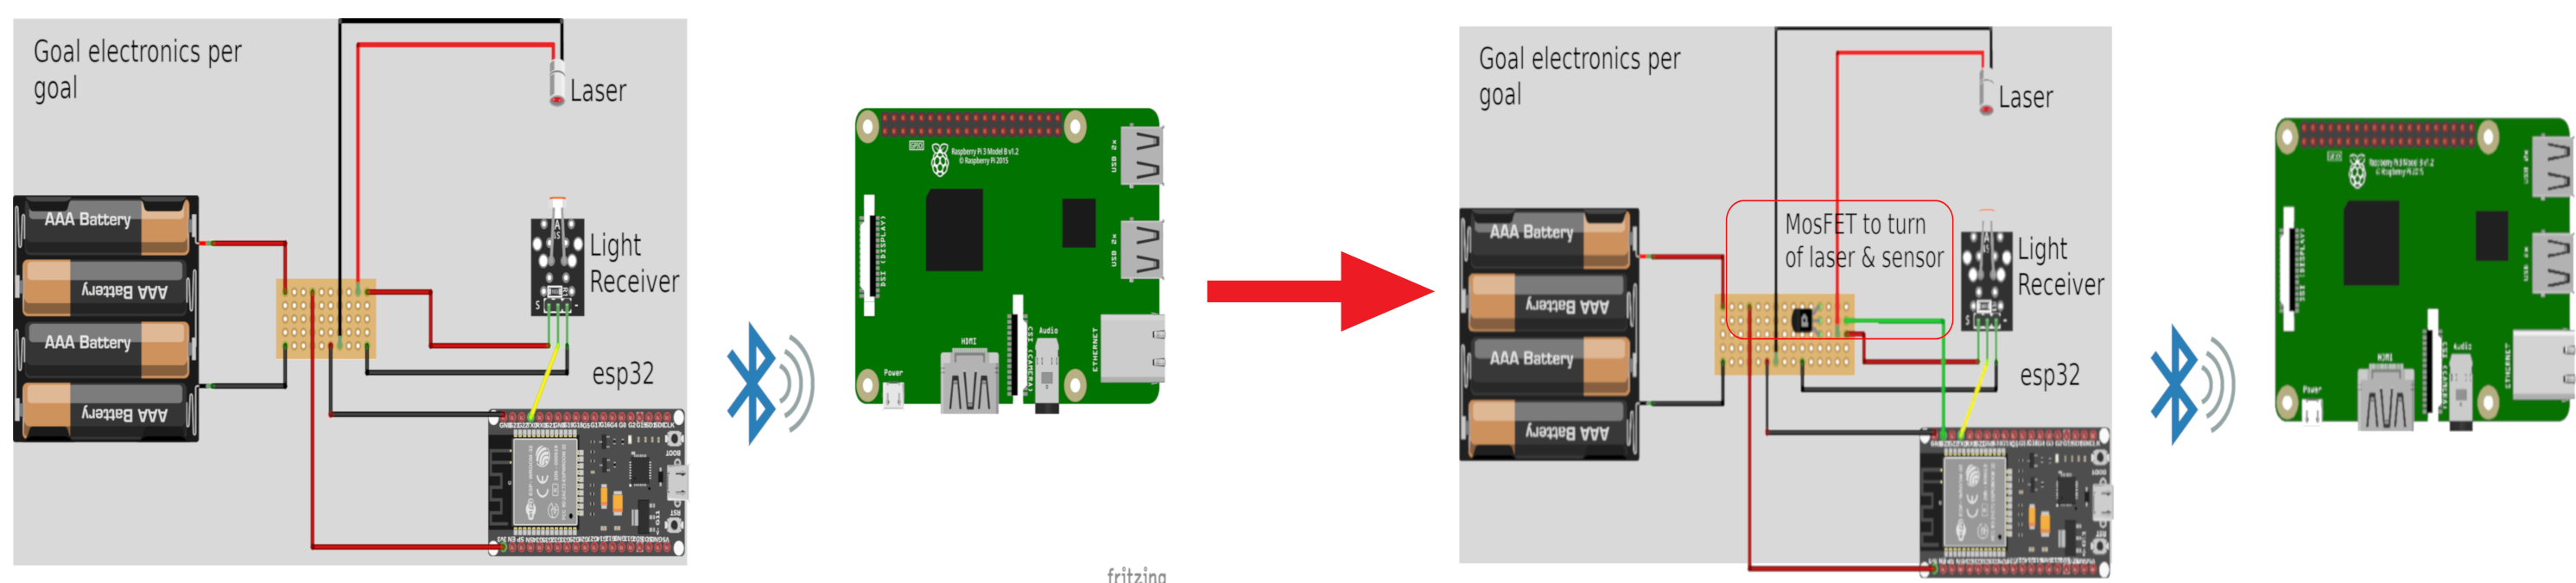
\includegraphics[scale=0.5]{figures/goal-parallel-series.png}
    \caption{The Goal Design, becoming smart}\label{fig:smartGoalDesign}
\end{figure}

Hardware is hard and expensive to update, but software can be easily changed and it is cheap to do so. Closing the circle, to have a smart table we need to be able to easily modify the software running on it. With OTA updates and orchestrated edge devices, we think this is possible to do, even on a big scale.
